% This file was created with tikzplotlib v0.10.1.
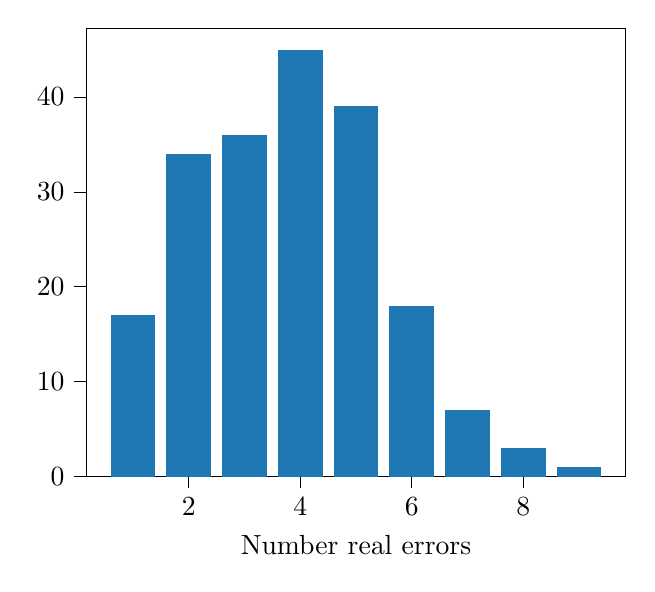
\begin{tikzpicture}

\definecolor{darkgray176}{RGB}{176,176,176}
\definecolor{steelblue31119180}{RGB}{31,119,180}

\begin{axis}[
tick align=outside,
tick pos=left,
x grid style={darkgray176},
xlabel={Number real errors},
xmin=0.16, xmax=9.84,
xtick style={color=black},
y grid style={darkgray176},
ymin=0, ymax=47.25,
ytick style={color=black}
]
\draw[draw=none,fill=steelblue31119180] (axis cs:0.6,0) rectangle (axis cs:1.4,17);
\draw[draw=none,fill=steelblue31119180] (axis cs:1.6,0) rectangle (axis cs:2.4,34);
\draw[draw=none,fill=steelblue31119180] (axis cs:2.6,0) rectangle (axis cs:3.4,36);
\draw[draw=none,fill=steelblue31119180] (axis cs:3.6,0) rectangle (axis cs:4.4,45);
\draw[draw=none,fill=steelblue31119180] (axis cs:4.6,0) rectangle (axis cs:5.4,39);
\draw[draw=none,fill=steelblue31119180] (axis cs:5.6,0) rectangle (axis cs:6.4,18);
\draw[draw=none,fill=steelblue31119180] (axis cs:6.6,0) rectangle (axis cs:7.4,7);
\draw[draw=none,fill=steelblue31119180] (axis cs:7.6,0) rectangle (axis cs:8.4,3);
\draw[draw=none,fill=steelblue31119180] (axis cs:8.6,0) rectangle (axis cs:9.4,1);
\end{axis}

\end{tikzpicture}
